\documentclass[10pt,letterpaper]{article}

\usepackage[T1]{fontenc}
\usepackage[utf8]{inputenc}
\usepackage[english]{babel}
\usepackage{mathptmx}
\usepackage[scaled=0.92]{helvet}
\usepackage{amsmath}
\usepackage{amssymb}
\usepackage[letterpaper,top=0.65in,bottom=0.72in,left=0.78in,right=0.78in,
  headheight=14pt]{geometry}
\usepackage[protrusion=true,expansion=true]{microtype}
\usepackage{xspace}
\usepackage[table]{xcolor}
\usepackage{graphicx}
\usepackage{booktabs}
\usepackage{colortbl}
\usepackage{etoolbox}
\usepackage{tabularx}
\usepackage{array}
\usepackage{enumitem}
\usepackage{float}
\usepackage{caption}
\usepackage{fancyhdr}
\usepackage{titlesec}
\usepackage[most]{tcolorbox}
\usepackage[round,authoryear]{natbib}
\usepackage[colorlinks=true,allcolors=argusblue]{hyperref}

% Anime-editorial paper palette derived from the mountain illustration: navy
% linework, cream paper, restrained blue, sand, and sage accents.
\definecolor{sjtuRed}{HTML}{C8161D}
\definecolor{argusblue}{HTML}{315BCE}
\definecolor{argusdeep}{HTML}{24465D}
\definecolor{ink}{HTML}{24465D}
\definecolor{muted}{HTML}{66717D}
\definecolor{papercream}{HTML}{FBF7EE}
\definecolor{papersand}{HTML}{F5E6C8}
\definecolor{papersage}{HTML}{6F9B86}
\definecolor{papergold}{HTML}{D9C58F}
\definecolor{mist}{HTML}{F8F2E7}
\definecolor{rulegray}{HTML}{D8E0E8}
\definecolor{softgray}{HTML}{FFFDF8}

% Canonical product name; use \MakeUppercase{\systemname} only where the
% surrounding typography requires all caps.
\newcommand{\systemname}{Argus\xspace}

\hypersetup{
  pdftitle={\systemname: A General-Purpose Agentic Runtime for Long-Horizon Reasoning},
  pdfauthor={Argus Team},
  pdfsubject={\systemname Technical Report},
  pdfkeywords={objective revision, verification-gated review, long-horizon research, general-purpose agentic runtime, persistent state}
}

\color{ink}
\setlength{\parindent}{1.05em}
\setlength{\parskip}{0pt}
\setlength{\textfloatsep}{12pt plus 2pt minus 2pt}
\setlength{\intextsep}{9pt plus 2pt minus 2pt}
\setlength{\floatsep}{8pt plus 2pt minus 2pt}
\setlength{\abovecaptionskip}{4pt}
\setlength{\belowcaptionskip}{0pt}
\renewcommand{\arraystretch}{1.10}
\setlist{leftmargin=1.45em,itemsep=1.5pt,topsep=3pt,parsep=0pt}
\setlength{\emergencystretch}{2.5em}
\AtBeginEnvironment{table}{\rowcolors{2}{papercream}{white}\arrayrulecolor{rulegray}}
\AtEndEnvironment{table}{\rowcolors{2}{white}{white}\arrayrulecolor{black}}

\titleformat{\section}
  {\sffamily\Large\bfseries\color{ink}}
  {\color{argusblue}\thesection}{0.65em}{}
\titleformat{\subsection}
  {\sffamily\large\bfseries\color{ink}}
  {\thesubsection}{0.55em}{}
\titleformat{\subsubsection}
  {\sffamily\normalsize\bfseries\color{ink}}
  {\thesubsubsection}{0.5em}{}
\titlespacing*{\section}{0pt}{1.15em}{0.45em}
\titlespacing*{\subsection}{0pt}{0.85em}{0.28em}
\titlespacing*{\subsubsection}{0pt}{0.65em}{0.2em}

\captionsetup{
  font=small,
  labelfont={bf,sf,color=ink},
  textfont={color=ink},
  labelsep=period
}

\pagestyle{fancy}
\fancyhf{}
\renewcommand{\headrulewidth}{0.35pt}
\fancyhead[L]{\footnotesize\rmfamily\color{muted}\systemname}
\fancyhead[R]{\footnotesize\rmfamily\color{muted}24$\times$7 Self-Evolving Agent System}
\fancyfoot[C]{\footnotesize\sffamily\color{muted}\thepage}
\fancypagestyle{firstpage}{
  \fancyhf{}
  \renewcommand{\headrulewidth}{0pt}
  \fancyfoot[C]{\footnotesize\sffamily\color{muted}\thepage}
}

\newtcolorbox{abstractbox}{
  enhanced,
  colback=papercream,
  colframe=papergold,
  boxrule=0pt,
  arc=1.5pt,
  left=9pt,right=9pt,top=7pt,bottom=7pt,
  before skip=7pt,after skip=6pt
}

\newtcolorbox{paperbox}[1]{
  enhanced,
  colback=softgray,
  colframe=papergold,
  boxrule=0.45pt,
  arc=1.5pt,
  left=8pt,right=8pt,top=6pt,bottom=6pt,
  before skip=6pt,after skip=6pt,
  fonttitle=\sffamily\bfseries\small\color{argusdeep},
  title={#1}
}

\newcommand{\code}[1]{\texttt{\small #1}}
\newcommand{\strong}[1]{\textbf{#1}}
\input{figures/swebench_metrics}
\input{figures/reviewer_metrics}
\input{figures/paper_case_study_metrics}

\begin{document}
\thispagestyle{firstpage}

\vspace{0.04in}

\noindent{\sffamily\small\bfseries\color{muted}
  \MakeUppercase{\systemname} TECHNICAL REPORT \enspace\textperiodcentered\enspace AUG 2026}\par
\vspace{0.12in}

\noindent{\raggedright\sffamily\fontsize{23}{26}\selectfont\bfseries\color{ink}
  \systemname: A General-Purpose Agentic Runtime\par
  for Long-Horizon Reasoning}\par
\vspace{0.07in}
\noindent{\raggedright\sffamily\fontsize{13}{16}\selectfont\bfseries\color{argusdeep}
  Verification-Guided Persistence, Pivoting, and Runtime Self-Evolution}\par
\vspace{0.08in}
\noindent{\raggedright\sffamily\normalsize\bfseries\color{ink}
  Argus Team}\par
\vspace{0.10in}

\noindent
\begin{minipage}[c]{0.28\linewidth}
  
\includegraphics[width=1.62in]{assets/microsoft-logo.png}
\end{minipage}%
\hfill
\begin{minipage}[c]{0.52\linewidth}
  \makebox[\linewidth][r]{%
    
\includegraphics[height=0.43in]{assets/sjtu-logo.png}\hspace{0.08in}%
    \raisebox{0.08in}{\sffamily\small\bfseries Shanghai Jiao Tong University}}
\end{minipage}

\begin{abstractbox}
\small
\textbf{Abstract.}
Long-horizon reasoning is not a race to push farther along a fixed route. A capable
runtime must persist while evidence supports the current approach, but pivot when
measurements expose a failed route, hidden constraint, or misspecified objective.
Because unrestricted pivoting is indistinguishable from rationalized failure, a
change of direction must be evidence-backed, admitted through a role-separated gate,
and recorded with its justification. We present \systemname, a persistent runtime
organized around Manager, Planner, Engineer, and Reviewer over bounded missions and
durable project state. A compact report-level model represents the working contract
as $K_t=(\iota,o_t,c_t,v_t)$ and explicit user decision state as $X_t$;
\code{ManagerAdmit} denotes the evidence-and-authority gate for material refinement.
These are analytical projections over current runtime surfaces, not one atomic API.
Reviewer-gated outcomes feed fixed-model runtime self-evolution, so a verified pivot
retains prior learning rather than resetting the campaign. After initial assignment,
ordinary rounds can run unattended while operator-owned decisions remain explicit
escalation points. Using GPT-5.5, we report task-native outcomes across seven benchmark
arenas. On SWE-Bench Pro, Direct Copilot with GPT-5.5/xhigh reaches approximately
\SWEProDirectAccuracy\% accuracy; \systemname reaches approximately
\SWEProArgusAccuracy\% while using \SWEProTokenRatio$\times$ the aggregate Tokens.
The same run supports an observational analysis of fixed-model runtime
self-evolution: reviewed updates accumulate in memory, skills, procedures,
verification state, and routing while the model parameters remain fixed.
Relative to the W1--6 startup window,
the mature W19--22 window uses \SWEProTokenReduction\% fewer solve input tokens and
\SWEProTimeReduction\% less active workflow time per task. The trajectory is not
monotone: task-composition shifts and late difficult-task Waves produce visible reversals.
Reviewer feedback requests revision on \ReviewerRevisionRequested{} tasks;
\ReviewerVerifierRecovered{} later pass the official verifier and
\ReviewerStrictRescues{} complete the strict review-loop rescue.
A complementary mathematical trace follows one objective across recovery, route
rejection, proof production, revision, acceptance, and the next mission. Together,
the benchmark trajectory and vertical case connect runtime organization to
measured long-horizon behavior. A six-project paper-production case study further
reconstructs \PaperCaseCampaignHours{} campaign-hours and six final manuscripts.
Its representative 163.6-hour trace turns seven rejected method routes into a
4,500-row negative-results study, then survives two submission-stage rollbacks
before completion. The retained trajectories also form structured training data
for future supervised and reinforcement learning.
\end{abstractbox}

\noindent
\begin{minipage}[t]{0.66\linewidth}
  \footnotesize\color{muted}
  \textbf{Keywords:} verified pivoting; runtime self-evolution; long-horizon
  research; general-purpose agentic runtime; persistent state.
\end{minipage}%
\hfill
\begin{minipage}[t]{0.31\linewidth}
  \raggedleft\small\sffamily\color{argusdeep}
  \textbf{Project:} \href{https://argusbot.cn/}{\textbf{argusbot.cn}}
\end{minipage}

\begin{figure}[H]
  \centering
  
\includegraphics[width=\linewidth]{figures/argus_teaser.pdf}
  \caption{\systemname runtime and breadth evidence. The central diagram shows
  Manager authority over tasks, research verticals, and Stage transitions;
  Planner, Engineer, and Reviewer operate over a shared workspace whose knowledge,
  event log, artifacts, backlog, budget, daemon, and memory persist across bounded
  missions. The surrounding cards report outcomes from seven task-native
  evaluations. Their bars use independent scales and indicate comparison direction
  with arrows; they are breadth evidence rather than a single normalized
  leaderboard.}
  \label{fig:overview}
\end{figure}

\section{Introduction}
\label{sec:introduction}

Long-horizon reasoning is not a longer version of one-shot question answering. At the
start of a mathematical investigation, neither the useful intermediate claims nor
the reachable theorem frontier may be known. An engineering user may express a
solution before understanding the actual performance, reliability, or integration
constraint. In system verification, a failed proof obligation may reveal a defect
in the implementation, an inconsistency in the specification, or a mistaken
assumption shared by both. In each case, execution changes what the user knows
about the problem itself.

This creates a different systems objective from autonomous completion of a fixed
prompt. The system must preserve a standing intent while allowing the operational
goal, constraints, and acceptance criteria to become more precise. It must value
verified intermediate progress---a counterexample, a stronger bound, a measured
bottleneck, a minimal failing trace, or a corrected specification---even when no
terminal artifact yet exists. It must also expose these updates to the user,
whose judgment can revise priorities and constraints for the next mission. The
system challenge is therefore not merely to persist, but to determine when evidence
supports continuing the current route and when it warrants a pivot in approach,
objective, constraints, or verification criteria.

Large language model agents have progressed from tool use and software execution to
complete research loops. ReAct, SWE-agent, and OpenHands established practical
interfaces between models and external environments
~\citep{yao2023react,yang2024sweagent,wang2024openhands}. The AI Scientist,
CycleResearcher, AutoSci, FARS, and Arbor extend this interaction into iterative
research programs covering different combinations of planning, experiments, review,
memory, and scientific
communication~\citep{lu2024aiscientist,weng2025cycleresearcher,qian2026autosci,
tang2026fars,jin2026arbor}. Their progress makes the central systems problem clear:
long execution becomes reasoning capability only when verified results accumulate
across iterations and the runtime can change direction when those results invalidate
the current route or task formulation.

In practice, long-running agents fail in four recurrent ways, consistent with
results showing that agent success declines as software-task horizons grow
~\citep{kwa2025longtasks}. First,
\emph{continuity} is fragile: a growing transcript is eventually compacted or
dropped, and later calls spend time reconstructing decisions that were already
made. Second, \emph{acceptance} is ambiguous when the component that performs the
work also declares it complete. Third, \emph{experience} is lost when only the
final artifact survives; failed branches, contaminated measurements, and useful
procedures disappear with the session that produced them. Hierarchical and
workflow-oriented memory systems address parts of this problem
~\citep{packer2023memgpt,wang2024workflowmemory,xu2025amem}. A larger context window
extends session continuity; durable institutional memory additionally requires
explicit state, ownership, and update rules.
Fourth, the task contract itself can be wrong or incomplete. A runtime that treats
the initial prompt, specification, or evaluator as immutable may optimize the wrong
quantity with increasing efficiency. Conversely, a runtime that freely rewrites
its objective turns learning into unauditable goal drift. The missing mechanism is
verified contract refinement: evidence must identify why a goal or constraint is
insufficient, and an authorized decision must record what changed and what remains
invariant.

We present \systemname (Autonomous Research Generation and Understanding System), a
verification-centered runtime for persistent and pivot-capable long-horizon reasoning. Its
central abstraction is a sequence of \emph{bounded missions} executed against a
durable, revisable task contract.
Four model-driven roles divide authority: a Manager anchors the objective and
campaign state, a Planner selects the next units of work, an Engineer implements
and evaluates them, and a Reviewer inspects artifacts and run outputs before issuing
the completion verdict or identifying a contract-level contradiction. The user
remains outside the repetitive round loop but retains authority at consequential
boundaries. Manager-visible evidence, alternatives, and unresolved questions make
clarification possible when the correct goal or constraint cannot be settled by
artifacts alone. These roles operate across three planes---control,
execution, and records---so that scheduling, work, and record keeping remain
separable even though they participate in one continuous loop.

This report describes the system and evaluations available through August 4, 2026;
historical benchmark traces are reported under the configurations that produced
them.

The runtime is designed to accumulate two coupled forms of state without updating
the base model. First, it self-evolves the \emph{approach} between the current goal
and constraints: each Stage retains attempted routes, measurements, Reviewer
verdicts, accepted and rejected results, reusable skills, verifiers, and routing
decisions, so later missions begin from a changed search policy rather than merely
a longer transcript. Second, verified evidence can sharpen the user-facing task
contract: goals can be decomposed or reframed, constraints can be discovered or
corrected, and acceptance tests can be strengthened. Verifier-gated runtime
self-evolution is the engine that improves execution under the current contract.
Verification-guided pivoting changes that contract only when evidence exposes a
material mismatch; user clarification or authorization governs changes that cannot
be settled by task-native evidence alone.
The term \emph{dense intelligence} describes the corresponding design goal: keep
decision, execution, and verification connected over the research horizon rather
than concentrating useful reasoning into isolated bursts. Section~\ref{sec:problem}
formalizes this conversion and the experiments measure its operating factors.

We sharpen this design language into a verified-progress theory. The final artifact
is a projection of a richer typed trajectory; intermediate states can carry
task-native value; reviewed compression retains the parts needed for later
decisions; and an accepted update counts as compounding only when it reduces future
task risk or resource cost. Contract refinement is admissible only when it preserves
the standing intent, cites new evidence, records the changed assumptions, and passes
the appropriate user or Manager authority boundary. This separates a justified
pivot from goal drift.

We evaluate the resulting system across seven benchmark arenas covering software
repair, GPU kernels, language-model training, training speed, research-assistant
tasks, and mathematical data synthesis. Beyond the headline SWE-Bench result, the
suite includes 76.8\% on AARRI-Bench and a 28.0 mathematical-data gap, both above
their reported references. SWE-Bench Pro is one row in this benchmark suite; its
731-task trajectory additionally enables analyses of Skill/Wiki evolution and
Reviewer intervention. A de-duplicated inventory records 41 research artifacts
across six programs as a separate breadth measure. We additionally report one
mathematical campaign as a representative vertical trace, showing how the four
roles hand off the same objective through recovery, route testing, proof
production, revision, acceptance, and retained state; it preserves one falsified
route and six proof-backed theorem-frontier updates. Finally, we reconstruct six
Argus paper-production campaigns spanning 254 missions and 16 Stage rollbacks from
their structured Stage and role logs. These traces are especially relevant to
pivoting because several initial positive hypotheses fail and become narrower
diagnostic or negative-results contributions through evidence-backed rollback.

This report makes seven contributions:

\begin{enumerate}[label=\textbf{C\arabic*.}]
  \item We formulate long-horizon reasoning as verified progress over a revisable task
    contract $K_t=(\iota,o_t,c_t,v_t)$ comprising standing intent, objectives, constraints, and
    verification criteria, rather than completion against an immutable prompt.
  \item We introduce a role-separated runtime for verification-guided persistence and pivoting that
    combines durable intent, bounded execution, independent review, user-visible
    contract refinement, append-only records, and fixed-model runtime evolution.
  \item We report one unified table across seven benchmark arenas, preserving each
    benchmark's backbone, backend, protocol, native metric, and reference.
  \item We analyze the SWE-Bench Pro row in depth: \systemname reaches approximately
    78\% accuracy versus 59\% for Direct Copilot at 1.41$\times$ aggregate Tokens;
    mature Waves are more efficient, and Reviewer intervention yields 34 verifier
    recoveries and 22 strict review-loop rescues.
  \item We reconstruct one mathematical campaign as a role-resolved Agent trace,
    showing why falsified routes and intermediate theorem-frontier updates are
    valuable before a terminal proof and how they reshape subsequent work.
  \item We present a six-project autonomous paper-production case study covering
    \PaperCaseCampaignHours{} campaign-hours, \PaperCaseRounds{} Engineer rounds,
    \PaperCaseContinues{} Reviewer revisions, and \PaperCaseRollbacks{} Stage
    rollbacks, with all six canonical pipelines reaching submission completion. A
    representative campaign uses seven verified no-go decisions to reframe a failed
    method search as a 4,500-row negative-results study, then repairs two late
    submission defects without discarding the accumulated research state.
  \item We document two artifact-level outcomes: a human-reviewed
    TileLang kernel merged into Flash Linear Attention and the operator-reported
    ACE-1 NPU prototype, while keeping their distinct evidence levels explicit.
\end{enumerate}

The remainder of the report follows a conventional research-paper organization.
Section~\ref{sec:related} positions the system against prior agent and autonomous
research work. Section~\ref{sec:problem} formalizes the operating problem;
Section~\ref{sec:method} presents the runtime; Sections~\ref{sec:methodology} and
\ref{sec:results} describe the evaluation protocol and results; and
Sections~\ref{sec:discussion}--\ref{sec:conclusion} discuss interpretation,
limitations, and conclusions. The appendix contains detailed experimental tables
and notation.

\section{Related Work}
\label{sec:related}

\subsection{Tool-Using and Software-Engineering Agents}

Language-agent research established the core loop of selecting actions, invoking
external tools, and conditioning later decisions on observations. Toolformer learns
when to call tools from self-supervised data~\citep{schick2023toolformer}, while
ReAct interleaves textual reasoning with environment actions~\citep{yao2023react}.
For repository-scale work, SWE-agent emphasizes the importance of an
agent-computer interface~\citep{yang2024sweagent}, and OpenHands provides an open
platform for generalist software-development agents~\citep{wang2024openhands}.

Evaluation has moved correspondingly from isolated code generation toward
interactive tasks. SWE-bench draws problems from real GitHub issues
~\citep{jimenez2024swebench}; AgentBench evaluates agents across heterogeneous
interactive environments~\citep{liu2023agentbench}; and AgentBoard adds
fine-grained progress analysis rather than reporting only final success
~\citep{ma2024agentboard}. Time-horizon studies further show that performance on
software tasks degrades as task duration increases~\citep{kwa2025longtasks}. These
results motivate treating long-horizon capability as a property of the complete
runtime, not only the model that generates the next action.

\subsection{Persistent Memory and Experience Reuse}

Several lines of work externalize experience beyond a single context window.
Generative Agents combine stored observations, reflection, and retrieval for
multi-day simulated behavior~\citep{park2023generative}. Reflexion retains verbal
feedback across attempts~\citep{shinn2023reflexion}, and Voyager accumulates an
executable skill library during open-ended interaction~\citep{wang2023voyager}.
MemGPT frames context management as a hierarchy of memory tiers
~\citep{packer2023memgpt}. More recent systems induce reusable task workflows
~\citep{wang2024workflowmemory} or organize memories through agentic linking and
retrieval~\citep{xu2025amem}.

\system{} shares the premise that useful experience should survive a model call,
but couples retention to explicit review. The Engineer may propose
a checkpoint or procedure; the Reviewer commits the canonical retained form after
inspecting artifacts and execution logs. This makes memory not only retrievable
but also attributable, versioned, and reversible.

\subsection{Autonomous Research and Program Search}

Automated research systems increasingly connect idea generation, implementation,
experimentation, and scientific communication. The AI Scientist presents an
end-to-end scientific-discovery pipeline~\citep{lu2024aiscientist}; Agent Laboratory
organizes specialized agents as research assistants~\citep{schmidgall2025agentlab};
and AIDE explores machine-learning improvements through iterative code search
~\citep{jiang2025aide}. The AI Scientist-v2 introduces agentic tree search over
research plans and experiments~\citep{yamada2025aiscientistv2}. Arbor similarly
uses a persistent hypothesis tree, a long-lived coordinator, and isolated executors
to make research cumulative~\citep{jin2026arbor}.

Executable evaluation can also drive discovery without reproducing a conventional
scientific workflow. FunSearch evolves programs against objective functions and
has produced new mathematical constructions~\citep{romera2024funsearch};
AlphaEvolve extends evolutionary code improvement to scientific and systems
problems~\citep{novikov2025alphaevolve}. These systems demonstrate the value of a
hard evaluator and repeated proposal--execution--selection cycles. \system{} focuses
on the more general runtime substrate around such cycles: persistent intent,
bounded missions, result admission, restartability, and reusable state across
heterogeneous research programs.

\subsection{Benchmarks for Research Agents}

Research-agent evaluation is beginning to cover realistic machine-learning and
scientific work. MLE-bench packages Kaggle competitions as machine-learning
engineering tasks~\citep{chan2024mlebench}; RE-Bench compares agents and human
experts in open-ended research-engineering environments~\citep{wijk2024rebench};
AARRI-Bench evaluates research-lifecycle tasks for models and harnesses
~\citep{wang2026aarri}; and AIRS-Bench targets frontier research-science agents
across a suite of scientific tasks~\citep{lupidi2026airsbench}. Together these
benchmarks emphasize held-out evaluation, task-native metrics, trajectories, and
resource controls.

The present report is complementary but weaker as a causal evaluation. It aggregates
public results produced under different protocols and distinguishes artifact-linked
records from website snapshots. This supports claims about
operational breadth and individual task outcomes, while leaving common-budget
comparisons and component ablations to future work.

\section{Problem Formulation}
\label{sec:problem}

\subsection{Dense-Intelligence Tasks}

The public Argus formulation defines a \emph{dense-intelligence task} as one that
sustains high-frequency reasoning, tool use, verification, and iteration across a
continuous time window until it produces a measurable result~\citep{argus_site}.
Three conditions determine whether a task has this shape:

\begin{enumerate}[label=\textbf{T\arabic*.}]
  \item \textbf{Invention.} The answer is not directly retrievable from a manual or
    database; it must be discovered through search and feedback.
  \item \textbf{Long horizon.} One pass is insufficient. Progress requires many
    dependent iterations over hours or days.
  \item \textbf{Verifiability.} A task-native evaluator can distinguish genuine
    improvement from a persuasive but incorrect claim.
\end{enumerate}

The defining loop is therefore proposal $\rightarrow$ execution $\rightarrow$
measurement $\rightarrow$ revised proposal. Performance engineering, security
research, scientific search, and quantitative research differ in domain but share
this operational structure. The task definition excludes both open-ended ideation
without an evaluator and fixed workflows that require time but no new decisions.

We model a campaign by an objective $o$, an initial artifact $y_0$, an evaluation
procedure $f$, and a resource budget $B$. The artifact may be code, a model, a
dataset, an experimental harness, a proof, or a manuscript. The campaign is divided
into bounded missions indexed by $t$, each producing

\begin{equation}
  \tau_t=(s_t,a_t,y_t,e_t,r_t),
  \label{eq:trajectory}
\end{equation}

where $s_t$ is the mission state, $a_t$ the actions taken, $y_t$ the resulting
artifact state, $e_t$ the observed measurements, and $r_t$ the review outcome. A mission
must terminate, pause, or transfer control explicitly; continuity belongs to the
persistent campaign state rather than an unbounded model session.

\subsection{Dense-Intelligence Density}

The website expresses useful intelligence per unit wall-clock time as

\begin{equation}
  \rho_I(T)
  =\frac{1}{T}\int_0^T
  \dot N_{\mathrm{tok}}(t)\,
  \eta_r(t)\,\eta_a(t)\,\eta_v(t)\,dt.
  \label{eq:dense-density}
\end{equation}

$\dot N_{\mathrm{tok}}(t)$ is the instantaneous rate of token-mediated reasoning
and action. The factors $\eta_r(t)$, $\eta_a(t)$, and $\eta_v(t)$ represent the
fractions converted into relevant reasoning, effective action, and valid
verification. The product is intentionally stricter than token throughput: a run
that repeatedly reads the same state, emits activity without changing an artifact,
or accepts unchecked claims can consume many tokens while contributing little to
$\rho_I$.

The public page summarizes the intended continuous-utilization advantage over a
fixed 48-hour window as

\begin{equation}
  \rho_I^{\mathrm{Argus}}(48\mathrm{h})
  \gg
  \rho_I^{\mathrm{human}}(48\mathrm{h}).
  \label{eq:density-hypothesis}
\end{equation}

Equation~\ref{eq:density-hypothesis} is a public design hypothesis, not a measured
result in this report. It refers to the density of sustained work over continuous
time, not to unconditional superiority of any individual reasoning step. Neither
$\rho_I$ nor its conversion factors are instrumented as a benchmark score in the
current evaluation.

\subsection{Online Life and Runtime Evolution}

The second website object separates model parameters from the operating state
around the model:

\begin{equation}
  \begin{aligned}
    H_{t+1} &= U(H_t,\tau_t,E_t), \\
    \theta_{t+1} &= \theta_t.
  \end{aligned}
  \label{eq:runtime-update}
\end{equation}

with the public state definition

\begin{equation}
  H_t=\left\{\text{Memory},\text{Skills},\text{Tools},
  \text{Verifiers},\text{Routing}\right\}.
  \label{eq:website-state}
\end{equation}

$E_t$ is the subset of results admitted from mission $t$. The equality for
$\theta$ is a scope condition: online evolution does not require a gradient update
to the underlying model. Section~\ref{sec:method} refines $H_t$ into named ownership
surfaces and tracks task/evaluation definitions as an additional component $Q_t$.
The update $U$ is partial; many missions change only memory, and some change no
reusable component.

\subsection{Capability-Set Expansion}

Let $C_t$ denote the effective capability set available at time $t$. The website
writes review-gated admission and the desired breadth/depth behavior as

\begin{equation}
  \begin{aligned}
    C_{t+1}
      &= C_t\cup\{c:\operatorname{Verify}(c,E_t)\geq\epsilon\}, \\
    W_{t+1} &\geq W_t,
    & D_{t+1}(d) &\geq D_t(d).
  \end{aligned}
  \label{eq:ood-expansion}
\end{equation}

where $W_t$ is frontier width across domains and $D_t(d)$ is depth within domain
$d$. The inequalities are retention desiderata over validated capability, not an
empirical guarantee that every run improves the system. Skills can become stale,
verifiers can be revised, and performance can regress on harder instances. A
negative result can still add value by excluding a failed branch even when the
effective capability set does not grow.

\subsection{Research Value}

Dense activity matters only when it produces new, valid, reusable information. The
website therefore defines the accumulated research value over horizon $T$ as

\begin{equation}
  V_R(T)
  =\int_0^T
  \rho_I(t)\,\Delta I(t)\,p_{\mathrm{valid}}(t)\,
  \eta_{\mathrm{reuse}}(t)\,dt,
  \label{eq:research-value}
\end{equation}

where $\Delta I(t)$ is information gain, $p_{\mathrm{valid}}(t)$ is the probability
that the claimed increment survives review, and
$\eta_{\mathrm{reuse}}(t)$ is the fraction that remains useful for later work.
Equation~\ref{eq:research-value} explains why token volume alone is not the product:
research value collapses if the work is repetitive, invalid, or non-reusable. It is
a conceptual objective, not a calibrated monetary or benchmark metric in this
report.

\subsection{The Information Advantage of Process Data}

Finally, the public formalization distinguishes the accepted artifact from the
trajectory that produced it:

\begin{equation}
  D_{\mathrm{process}}
  =\{(s_k,a_k,e_k,r_k,\Delta H_k)\}_{k=1}^{N}
  \supsetneq
  D_{\mathrm{final}}=\{y^\star\}.
  \label{eq:process-data}
\end{equation}

The process record contains states, actions, measurements, review feedback, and
runtime-state changes, including failed branches omitted from $y^\star$. This
additional information can reduce repeated search, support later analysis, and provide
grounded material for later skill construction or evaluation. \system{} retains
typed, credential-redacted observations and verdicts, not private chain-of-thought
transcripts.

\section{\systemname Runtime}
\label{sec:method}

\subsection{System Overview}

\systemname is a verification-centered runtime built around a user, four
model-driven roles, and three system planes. The user supplies standing intent,
domain judgment, and authority over material tradeoffs. The \emph{control plane}
turns that intent into a durable task contract and schedules work; the
\emph{execution plane} performs one bounded mission against real tools and
artifacts; and the \emph{record plane} stores evidence, decisions, and contract
history without deciding whether the work is scientifically complete. The
distinction is operational: control owns scheduling and contract transitions,
execution owns work and mission review, and the record plane owns the immutable
record but no completion decision.

The four roles divide research authority as summarized in
Table~\ref{tab:roles}. The Manager spans the campaign rather than one execution
round. The Manager is also the user-facing boundary: it preserves standing intent,
surfaces consequential ambiguity, and commits authorized contract refinements. The
Planner authors future work and the Engineer performs it. Every normal mission
round then passes to a fresh independent Reviewer; historical
Engineer-self-review fields remain only for compatibility with older traces. The
interfaces are structured objects rather than untyped prose, which makes ownership
and recovery behavior explicit.

The notation $K_t$ is a report-level abstraction over persisted campaign identity,
objectives, Stage state, constraints, verifier obligations, and decision records.
The current implementation distributes these fields across runtime surfaces rather
than storing one monolithic object named $K_t$.

\begin{table}[H]
\centering
\small
\begin{tabularx}{\linewidth}{@{}p{1.6cm} p{4.0cm} X@{}}
\toprule
\rowcolor{papersand}
\textbf{Role} & \textbf{Primary responsibility} & \textbf{Authoritative output} \\
\midrule
Manager & Preserve standing intent; commit task contract, lifetime, route, and campaign stage & Contract refinement, user escalation, campaign division, and stage transition \\
Planner & Decompose the current verified frontier into bounded tasks and dependencies & Task specifications, plan status, verifier obligations, and stage checklist updates \\
Engineer & Modify artifacts, invoke tools, and run experiments for one round & Execution result, artifacts, measurements, and checkpoint handoff \\
Reviewer & Independently inspect every normal round against the current contract & \code{done}, \code{continue}, \code{blocked}, or \code{replan\_requested}; verified frontier update; contradiction or expert-question report \\
\bottomrule
\end{tabularx}
\caption{Authority separation in \systemname. The Engineer executes; a fresh
independent Reviewer controls admission after every normal mission round; Manager
owns contract and Stage transitions at the user-facing boundary.}
\label{tab:roles}
\end{table}

\begin{paperbox}{Algorithm 1: Reviewed mission loop}
\small
\begin{tabbing}
\quad\=\quad\=\quad\=\kill
\textbf{Input:} standing intent $\iota$, contract $K_t$, user state $X_t$, runtime state $H_t$, backlog $B$, budget $b$ \\
$c \leftarrow \operatorname{ManagerCommit}(\iota,K_t)$; persist campaign identity and contract \\
\textbf{while} $b$ remains and $c$ is not complete \textbf{do} \\
\> $q \leftarrow \operatorname{Planner}(B,H_t,c)$; claim one bounded task \\
\> $\tau_t \leftarrow [\,]$ \\
\> \textbf{repeat} \\
\>\> $(y,e) \leftarrow \operatorname{Engineer}(q,H_t)$ \\
\>\> $r \leftarrow \operatorname{Reviewer}(K_t,q,y,e)$ \\
\>\> append $(q,y,e,r)$ to $\tau_t$ \\
\>\> \textbf{if} $r=\code{continue}$ \textbf{then} $q \leftarrow r.\code{next\_action}$ \\
\> \textbf{until} $r\in\{\code{done},\code{blocked},\code{paused},\code{replan\_requested}\}$ \\
\> $E_t \leftarrow \operatorname{AdmitResult}(e,r)$ \\
\> $X_{t+1} \leftarrow \operatorname{SurfaceEvidence}(X_t,E_t,r)$ \\
\> $K_{t+1} \leftarrow K_t$ \\
\> \textbf{if} $r=\code{replan\_requested}$ or contract refinement is proposed \textbf{then} \\
\>\> $K_{t+1} \leftarrow \operatorname{ManagerAdmit}(K_t,E_t,r,u_t)$ \\
\> $H_{t+1} \leftarrow U(H_t,\tau_t,E_t,K_{t+1})$; persist outcome, trace, contract, and state \\
\> $t \leftarrow t+1$; refill $B$ when required \\
\textbf{end while} \\
\textbf{Output:} accepted frontier, inspectable trajectory, refined task contract, and updated expert/runtime state
\end{tabbing}
\end{paperbox}

\subsection{Bounded Missions over Durable Contracts}

The long-lived object in \systemname is the campaign, not a provider transcript. A
campaign has a persisted identity, standing intent, current task contract, accepted
frontier, and explicit unresolved questions. Its work is divided into missions with
explicit outcomes. The scheduler assigns one mission at a time, records its result,
and advances only at a clean mission boundary. Mission assignment is transactional,
preventing duplicate work under concurrency, and resumed execution is tied to the
persistent campaign identity.

Engineer and Reviewer calls use fresh provider sessions for each round. Cross-session
continuity comes from an ordinary shared \code{CHECKPOINT.md} containing durable
state, evidence references, open questions, and the next step. This follows the
broader move from monolithic context toward managed memory tiers and reusable
workflows~\citep{packer2023memgpt,wang2024workflowmemory,xu2025amem}. The Engineer
updates the checkpoint after execution. The Reviewer then reads and corrects the
same file and is its final editor for that round. The full history remains in
artifacts and the event record.

This design makes restart and upgrade behavior part of the method. A running process
hands off only at a mission boundary, and the replacement resumes from the same
persistent campaign identity. After an interruption, replay or reassignment begins
from committed campaign state rather than reconstructing the task from a model
transcript.

The same persistence supports user interaction at a larger timescale. The user
does not need to repeat the original context or monitor every tool call. When a
Reviewer finds that the current verifier cannot distinguish alternatives, that a
constraint conflicts with observed reality, or that multiple valid tradeoffs remain,
the issue is surfaced with evidence and options. The resulting clarification is
committed through Manager into the durable contract. Later missions therefore begin
from the refined understanding rather than from either the original ambiguous prompt
or an agent-invented replacement goal.

\subsection{Autonomy between User Decision Boundaries}

The runtime does not require a human to supervise each round. The harness assigns
local authority to the four roles: Manager maintains the campaign and contract,
Planner creates bounded executable work, Engineer acts on real artifacts, and an
independent Reviewer decides whether evidence supports completion, continuation,
blocking, or replanning. Checkpoints, event history, task claims, external-job
state, and mission outcomes survive session replacement. Consequently, the runtime
can execute for long intervals without synchronous human input and surface a user
decision only when evidence exposes a material value tradeoff, missing information,
or operator-owned constraint.

This is stronger than adding a human-approval button. The autonomous path must
remain capable of selecting routes, running experiments, rejecting invalid work,
consolidating intermediate progress, and ending an unproductive mission. Human
input refines the campaign at consequential boundaries; it is not the mechanism
that keeps the ordinary loop alive.

\subsection{Verification as the Pivot Gate}

All role invocations pass through a common instrumentation layer that records usage
and associates each call with the mission trace. The Engineer and Reviewer share
the same artifact state, allowing review of the actual outputs and execution record
rather than only the Engineer's summary. A typed, append-only trace is the canonical
timeline; user interfaces are projections over that record.

The source of a mission completion verdict is explicit: a fresh Reviewer returns a
structured verdict after every normal Engineer round. Review evaluates more than
terminal completeness. It can admit a bounded frontier increment, reject an
unsupported claim, identify a faulty verifier or inconsistent specification,
request another experiment, or ask Manager to replan and surface a user decision.
Historical
\code{review\_source=engineer\_self\_review} values describe earlier runtime
versions and are retained only so longitudinal traces remain interpretable.
Completion never comes from filenames, Token volume, content hashes, or prose
keywords. The corresponding artifacts and execution records remain inspectable,
while credential redaction preserves the evidence boundary.

Verification is therefore the gate between persistence and pivoting. Agent
execution externalizes hypotheses into artifacts and measurements; Reviewer turns
those outputs into calibrated claims and unresolved alternatives; Manager presents
material choices in terms the user can inspect; and user judgment updates the
contract governing subsequent execution. Without verification, persistence can
compound error. Without persistent self-evolution, verification repeatedly finds
the same errors. Their combination converts a long trajectory into cumulative
problem understanding and reusable capability.

\subsection{Staged Approach Self-Evolution and Contract Pivoting}

Equation~\ref{eq:runtime-update} separates the model from the state around it.
Table~\ref{tab:runtime-ownership} identifies how each component can change and who
owns the committed update. The ownership model is intentionally not uniform. Memory
and skills use a work-versus-certification split: the Engineer or Scientist produces
a candidate, and the Reviewer commits the retained form. Tools and procedures are
system-configured. Stage checklists are Planner-owned, with Reviewer feedback rather
than a second commit gate. Routing policy is Manager-committed, while task
definitions are Planner-authored and scheduler-committed. The task contract is
different from all of these: evidence and Reviewer findings may propose a change,
Manager commits operational refinements, and the user retains authority
over standing intent and value-laden tradeoffs that evidence alone cannot settle.

We use verifier-gated runtime self-evolution to mean the staged evolution of the approach
used to move from the current objective toward satisfaction of the current
constraints. The underlying model parameters remain fixed, while reviewed missions
change the persistent search state available to later work. Each Stage maintains an
approach record $\Pi_t$ containing route hypotheses, actions, task-native evidence,
Reviewer verdicts, retained failures, and the next admissible frontier. A complete
update cycle has four parts:
(1) an execution trajectory produces a candidate memory, skill, procedure,
verification rule, routing decision, or task definition; (2) the responsible role
checks the candidate against artifacts and task-native evidence; (3) the authorized
owner commits, revises, or rejects the update; and (4) a later mission retrieves the
retained state as part of its starting context or execution policy. Activity that
does not survive this commit-and-reuse path is not counted as self-evolution.
Contract pivoting is distinct: it is the evidence-backed refinement of $K_t$ and
$X_t$, with user clarification or authorization where required. Neither mechanism implies that every
mission improves the system or changes the contract.

This preserves a strong self-evolution claim without conflating it with goal
mutation. $K_t$ defines the current objective, constraints, and verifier;
$\Pi_t$ records how the runtime has learned to navigate inside that envelope. If a
verified contract refinement changes the envelope, the prior approach record
remains staged evidence of which routes failed and which procedures or verifiers
remain reusable.

\begin{table}[H]
\centering
\small
\begin{tabularx}{\linewidth}{@{}p{2.25cm} p{2.75cm} p{2.55cm} X@{}}
\toprule
\rowcolor{papersand}
\textbf{State} & \textbf{Change source} & \textbf{Commit owner} & \textbf{Persistent form} \\
\midrule
$M$: memory & Engineer trajectory & Reviewer & Curated checkpoint and event-derived journal \\
$S$: skills & Engineer / Scientist & Reviewer & Versioned skill library \\
$A$: tools and procedures & System configuration & System configuration & Versioned tool and procedure registry \\
$V$: verification & Planner & Planner & Stage checklist; Reviewer supplies feedback \\
$R$: routing and roles & Runtime policy & Manager & Campaign routing policy \\
$Q$: tasks and evaluations & Planner & Scheduler & Backlog task specifications and scopes \\
$\Pi$: staged approach & Mission trajectories and Reviewer verdicts & Manager / Planner & Accepted frontier, rejected routes, route rationale, and next approach \\
$K$: task contract & User clarification, evidence, and Reviewer findings & Manager / user & Versioned intent, objective, constraints, verifiers, and provenance \\
\bottomrule
\end{tabularx}
\caption{Attributable ownership of persistent and revisable state. A mission usually updates only
a subset of these components; material changes to standing user intent are not
delegated to the runtime.}
\label{tab:runtime-ownership}
\end{table}

Two knowledge surfaces carry reusable experience. Versioned skills store procedures
that can be matched to later tasks. A project knowledge base stores source-linked
records and synthesized pages derived from reviewed outcomes. Neither surface is
treated as automatically correct: entries can be revised, archived, or retired when
later results contradict them.

This mechanism can improve a later mission without changing the model itself. A
retained failure can prevent a repeated dead end; a reviewed procedure can shorten
environment inspection; a verifier can reject a previously accepted shortcut; and
a routing update can assign independent review to a higher-risk task. The mechanism
does not imply monotonic improvement. Some missions commit no reusable state,
retained state can become stale, and a harder task distribution can increase cost
even after useful state has accumulated.

The user-facing benefit is complementary. A retained failure can show that a
requested optimization is physically or economically irrelevant; a stronger
verifier can expose that the original success metric was gameable; and a proof
counterexample can replace a vague conjecture with a sharper reachable frontier.
The runtime is not learning the user's preferences covertly. It is making the
evidence and tradeoffs explicit enough for those preferences to be stated and
revised deliberately.

\subsection{Reliability and Resource Governance}

Long-running systems fail through operational drift even when individual model
calls are strong. \systemname therefore combines round-level progress
classification with mission-boundary replanning. Work that repeatedly produces no
decision or artifact change is stopped or reformulated, while long-running external
jobs are tracked separately from model reasoning. These mechanisms bound execution;
scientific correctness remains with the task evaluator and independent Reviewer.

Short Planner DAG nodes expose a subtle control problem: their default three-round
budget is much smaller than the default absolute thresholds for semantic stall,
soft escalation, and hard escalation. The current runtime fits each enabled guard
to the reachable range when \code{max\_rounds} shrinks. For budget $m$, semantic
stall and soft escalation must satisfy $g\leq m-1$, while hard escalation may fire
on the final round and therefore satisfies $g\leq m$. Explicit zero still disables
a guard, and the default 500-round configuration is unchanged. A two-round budget
does not silently turn a configured multi-round stall detector into a one-strike
policy: the impossible detector is disabled unless the caller explicitly requests
threshold one. This coordination preserves meaningful stop and replan signals
instead of falling through silently to the generic maximum-round outcome.

These liveness guards do not decide scientific truth and do not freeze a mistaken
contract. They create bounded points at which Reviewer and Planner can distinguish
three cases: the current route is unproductive, the evidence frontier has advanced
but terminal work remains, or the task contract itself needs user-visible
refinement. This distinction is important because ``not done'' is not synonymous
with ``no progress,'' and ``cannot verify'' is not synonymous with ``incorrect.''

We call this property \emph{honest stopping}: the harness can end the current unit
of work without converting uncertainty, exhaustion, or an external dependency into
a success claim. The implementation keeps completion, incomplete research,
stalling, blocking, infrastructure blocking, failure, and operator interruption as
separate outcome dimensions. Reviewer may return \code{blocked} or
\code{replan\_requested}; a hard escalation ends the mission with a
planner-readable reason. Semantic stall accumulates only from the Reviewer's
explicit structured \code{forward\_progress=false}; a missing or malformed signal
is treated as unknown rather than inferred from prose or filesystem activity.
Stopping therefore preserves both epistemic honesty and the information needed to
resume, decompose, or change approach.

Resource accounting is centralized at model-call and external-job boundaries.
Budgets are checked before work begins and reconciled after completion, preventing
individual roles from expanding their own allocation. Concrete scheduling,
sandboxing, and deployment mechanisms are implementation choices rather than part
of the scientific claim.

\section{Empirical Methodology}
\label{sec:methodology}

The current evaluation is designed as a transparent empirical record rather than
a controlled ablation study. Recent research-agent benchmarks instead hold tasks,
evaluators, and time or resource budgets fixed to support direct comparisons
~\citep{chan2024mlebench,wijk2024rebench,wang2026aarri,lupidi2026airsbench}. The
The analysis asks whether the deployed runtime has produced competitive
artifacts across heterogeneous settings and how broadly it has been used.

\subsection{Research Questions}

We organize the evaluation around two questions.

\paragraph{RQ1: Cross-domain performance.}
What task-native results has \system{} produced across distinct benchmark arenas,
and how do those results compare with the human or paper-reported references
published for each arena?

\paragraph{RQ2: Research breadth.}
How many de-duplicated manuscripts and drafts has the research pipeline produced,
and how are they distributed across research programs?

The questions deliberately avoid causal language. Although all six runs use
GPT-5.5 through the Codex backend, the records do not share one task interface,
random-seed policy, evaluator, or hardware protocol. Consequently, they can
establish operational breadth and task-level outcomes, but not the isolated
contribution of role separation, checkpointing, review, or any other individual
mechanism.

\subsection{Benchmark Definitions}

Following the task-definition style used by Arbor~\citep{jin2026arbor}, we define
each arena by its research artifact, evaluator, native metric, and metric direction.
The common research-agent configuration is GPT-5.5 through Codex; the target
artifact and evaluator differ by arena.

\paragraph{NVIDIA SOL-ExecBench.}
SOL-ExecBench evaluates correctness-preserving optimization of real GPU kernels
against workload-specific hardware speed-of-light models~\citep{lin2026solexecbench}.
Candidate implementations must first match the reference output; performance is
then assessed relative to the hardware limit. The reported Argus result covers 101
B200 kernels and uses global rank, first-place finishes, and top-three placements as
the public summary; better rank and more high placements are better.

\paragraph{nanochat on B200.}
This arena instantiates the nanochat autoresearch task on one B200 GPU
~\citep{karpathy_nanochat,karpathy_autoresearch}. The editable artifact is the
training program, and each candidate receives a fixed five-minute training window.
The evaluator reports validation bits per byte (BPB), a tokenizer-independent
compression metric; lower BPB indicates a better trained model. The public record
summarizes 426 autonomous attempts.

\paragraph{nanochat on H100.}
The H100 arena uses the same five-minute training objective and lower-is-better BPB
metric, but executes on one H100 and therefore constitutes a separate
hardware-specific optimization problem. The public result summarizes a search over
37 implemented mechanisms. B200 and H100 values are compared only with references
measured under their corresponding hardware protocol, not directly with each other.

\paragraph{nanoGPT speedrun.}
NanoGPT-Bench measures the wall-clock time required for an eight-H100 training run
to reach the fixed validation-loss threshold of $3.28$~\citep{jordan_nanogptbench}.
A candidate is valid only when it reaches that target; among valid candidates,
lower training time is better. The reported value is the mean of $N{=}10$ verifier
runs for the selected artifact.

\paragraph{AARRI-Bench.}
AARRI-Bench evaluates models and agentic harnesses on granular tasks from the
research lifecycle, including research judgment and professional research
practice~\citep{wang2026aarri}. The Argus evaluation uses 82 research-intern tasks
and reports the number and percentage solved. Higher solve rate is better; the
paper-reported best is used as the external comparison.

\paragraph{Math-Reasoning Data Synthesis (Arbor AO suite).}
This row is the Math-Reasoning Data Synthesis task from Arbor's Autonomous
Optimization suite, not a generic benchmark named ``Arbor''~\citep{jin2026arbor}.
The editable artifact is a pipeline that generates AIME-style reasoning problems.
Arbor evaluates generated problems with a GPT-5.5 ReAct solver and reports the mean
$\mathrm{pass@4}-\mathrm{pass@1}$ gap: a larger gap rewards problems that are not
solved immediately but become solvable with additional attempts. The published
comparison uses Argus 28.0, Arbor 20.83, Claude Code 8.33, and Codex 6.25.

\subsection{Evaluation Sources}

The benchmark record is a snapshot of the six public result cards on the Argus
results page~\citep{argus_results}. It was retrieved on July 14, 2026 with the final
URL, HTTP status, and raw-page SHA-256 stored in
\srcpath{evidence/website\_results.json}. Each card preserves the arena, protocol,
reported result, comparison text, source URL, and corroboration status.

The research-output record is a de-duplicated inventory of the public Argus paper
collection~\citep{argus_research}, stored in
\srcpath{evidence/paper\_inventory.json}. It distinguishes manuscripts from drafts,
removes duplicate versions, and groups artifacts into six programs. The inventory
is not a publication-acceptance record and is not compared with the paper output of
other agents.

The two quantitative figures in Section~\ref{sec:results} are generated
deterministically from these JSON files. Structural diagrams are explanatory
illustrations; they are not empirical plots. Figure provenance is summarized in
Appendix~\ref{app:evidence-map}.

\paragraph{Provenance scope.}
Two rows---nanochat B200 and the nanoGPT speedrun---add artifact identifiers,
verifier excerpts, and content digests to the public result snapshot. The other four
rows preserve the public source and page hash but do not yet provide a complete
artifact bundle. This distinction limits reproducibility and is documented in
Appendix~\ref{app:evidence-map}; it is not an additional performance dimension.

\subsection{Metrics and Comparison Policy}

The six arenas use incompatible metrics: global rank, bits per byte, wall-clock
time, solve rate, and a source-reported gap value. We do not normalize these values
or average them into a single score. Each result is shown in its native unit with
its own protocol and comparison. Lower is better for bits per byte and wall-clock
time. For the Math-Reasoning Data Synthesis comparison, the Arbor task definition
identifies the mean $\mathrm{pass@4}-\mathrm{pass@1}$ gap as higher-is-better
~\citep{jin2026arbor}.

Human records and paper-reported bests are used when the public card provides them.
The SOL-ExecBench row instead uses global rank as its headline and retains the
source's system comparison as secondary context. No significance test is introduced
where the source record does not provide the underlying repeated measurements.

\subsection{Portfolio Counting Policy}

The paper inventory counts a research artifact once after duplicate versions are
removed. ``Manuscript'' and ``draft'' are artifact states, not peer-review outcomes.
The headline total therefore answers RQ2---how much research material the pipeline
produced across programs---but does not measure novelty, correctness, acceptance,
or scientific impact. Those questions require external review beyond the scope of
the current records.

\section{Results}
\label{sec:results}

\subsection{RQ1: Cross-Domain Performance}

Figure~\ref{fig:public-results} and Table~\ref{tab:public-results} report the six
public benchmark cards in their native units. The results span kernel optimization,
small-language-model training, training-speed optimization, research-assistant
tasks, and data synthesis. Because the protocols differ, the figure uses separate
panels and the table states the research-agent backbone and backend beside every
protocol and result.

\begin{figure}[H]
  \centering
  
\includegraphics[width=0.80\linewidth]{figures/public_results.pdf}
  \caption{Public results across six arenas. Each panel retains its task-native
  metric and identifies the GPT-5.5 backbone and Codex backend; values are not
  cross-normalized. The figure is
  generated from \srcpath{evidence/website\_results.json}.}
  \label{fig:public-results}
\end{figure}

\begin{table}[H]
\centering
\footnotesize
\renewcommand{\arraystretch}{1.16}
\begin{tabularx}{\linewidth}{@{}>{\raggedright\arraybackslash}p{2.05cm} >{\centering\arraybackslash}p{1.25cm} >{\centering\arraybackslash}p{1.05cm} >{\raggedright\arraybackslash}p{2.35cm} >{\raggedright\arraybackslash}p{1.55cm} X@{}}
\toprule
\textbf{Benchmark} & \multicolumn{2}{c}{\textbf{Research agent}} & \textbf{Hardware / protocol} & \textbf{Result} & \textbf{Comparison} \\
\cmidrule(lr){2-3}
& \textbf{Backbone} & \textbf{Backend} & & & \\
\midrule
SOL-ExecBench & GPT-5.5 & Codex & B200; 101 kernels & Global \#6; 2$\times$\#1; 7 top-3 & Two H2H wins over Recursive \\
nanochat B200 & GPT-5.5 & Codex & 5 min; 1$\times$B200; 426 attempts & 0.9636 BPB & Human SOTA 0.9646 \\
nanochat H100 & GPT-5.5 & Codex & 5 min; 1$\times$H100; 37 mechanisms & 0.9855 BPB & Human SOTA 0.9879 \\
nanoGPT speedrun & GPT-5.5 & Codex & 8$\times$H100; $N{=}10$ & 79.77 s & Same-device human \#83: 80.18 s \\
AARRI-Bench & GPT-5.5 & Codex & 82 research-intern tasks & 63/82 (76.8\%) & Paper best 68.3\% \\
Math-Reasoning Data (Arbor) & GPT-5.5 & Codex & AIME-style synthesis & 28.0 gap & Arbor 20.83; Claude 8.33; Codex 6.25 \\
\bottomrule
\end{tabularx}
\caption{Six public benchmark results~\citep{argus_results}. Backbone denotes the
research-agent model driving Argus; Backend denotes the agent execution surface,
not the target model or comparison system.}
\label{tab:public-results}
\end{table}

Several rows meet or exceed the reference printed on the corresponding public
card. On nanochat B200, the reported 0.9636 BPB is lower than the listed human SOTA
of 0.9646~\citep{karpathy_nanochat,karpathy_autoresearch}. On the nanoGPT speedrun,
79.77 seconds is below the same-device human record of 80.18 seconds
~\citep{jordan_nanogptbench}.
AARRI-Bench reports 63 of 82 tasks (76.8\%), compared with the card's paper-reported
best of 68.3\%~\citep{wang2026aarri}. The nanochat H100 value of 0.9855 BPB is lower
than the listed 0.9879 reference. The SOL-ExecBench headline is Global \#6 across
101 kernels, with two first-place head-to-head outcomes and seven top-three
outcomes, including the source-reported comparison with Recursive
~\citep{recursive2026firststeps}; SOL-ExecBench defines the hardware-limit-relative
evaluation used by the arena~\citep{lin2026solexecbench}. On the
Math-Reasoning Data Synthesis task, the higher-is-better pass gap is 28.0 for Argus,
compared with 20.83 for Arbor, 8.33 for Claude Code, and 6.25 for Codex
~\citep{jin2026arbor}.

These outcomes answer RQ1 at the level supported by the public record: \system{}
has produced competitive task-native artifacts across multiple research settings.
The common GPT-5.5/Codex configuration removes one source of ambiguity, but the
heterogeneous tasks, evaluators, and hardware protocols still prevent direct
cross-arena averaging or attribution to a particular runtime mechanism.

\subsection{RQ2: Research Breadth}

The public research inventory contains \textbf{41} de-duplicated artifacts:
\textbf{35 manuscripts} and \textbf{6 drafts} across six programs. The distribution
is shown in Figure~\ref{fig:portfolio}. Multimodal and
vision-language research is the largest program with 16 artifacts, followed by
cognitive-bias studies with 9 and efficiency, compression, and decoding with 7.

\begin{figure}[H]
  \centering
  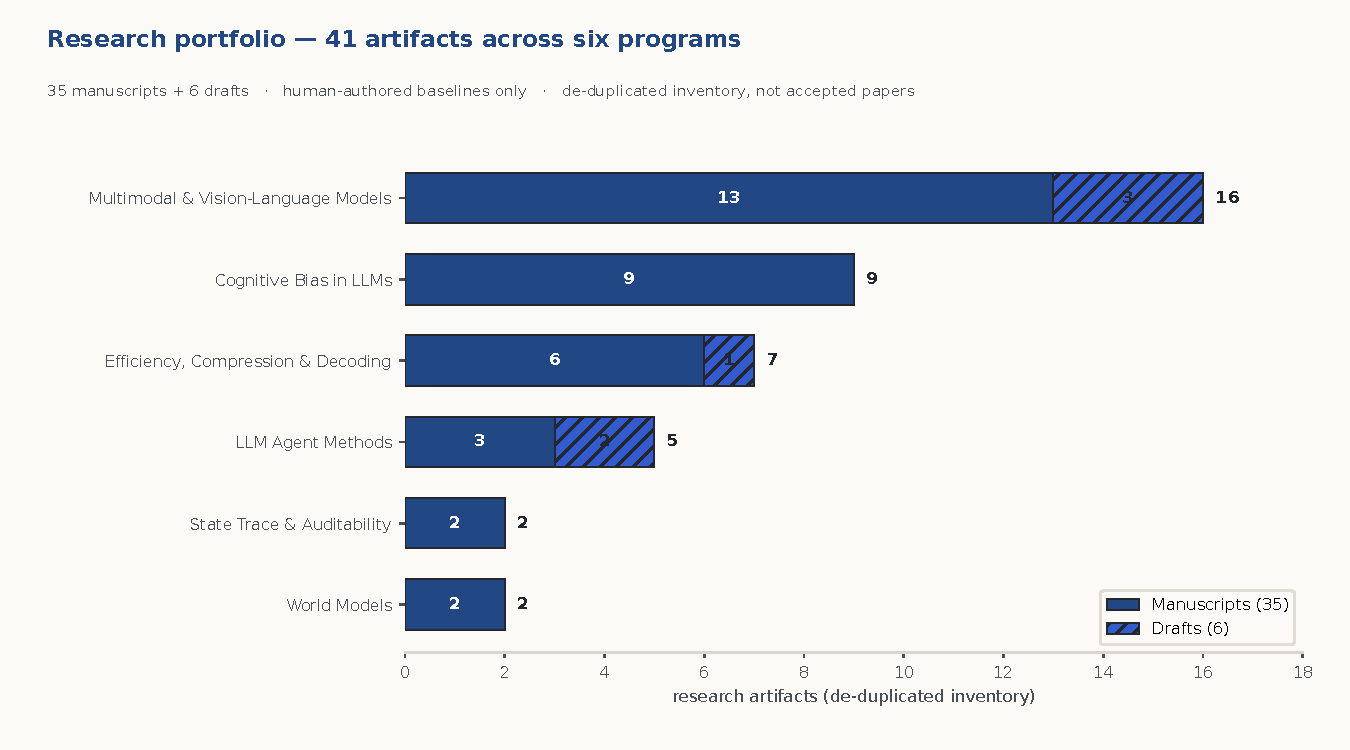
\includegraphics[width=0.70\linewidth]{figures/paper_portfolio.pdf}
  \caption{De-duplicated research-artifact inventory by program and status. The
  chart is generated from \srcpath{evidence/paper\_inventory.json}; manuscript and
  draft labels do not imply external acceptance.}
  \label{fig:portfolio}
\end{figure}

The inventory records sustained output and breadth across task
classes. It does not establish that all artifacts are novel, correct, accepted, or
of equal quality. The count is therefore reported as a production record rather
than a publication metric.

\input{sections/06b_vertical_trace}
\subsection{Autonomous Paper-Production Case Study}
\label{sec:paper-case-study}

The benchmark suite evaluates task endpoints, while the mathematical trace follows
one research objective in depth. A complementary question is whether the same
runtime can carry multiple research programs through the complete paper-production
lifecycle. We therefore reconstruct six projects spanning evaluation reliability,
vision--language matching, test-time adaptation, GUI agents, multimodal
hallucination, and model quantization. The initial objectives and compute
environments were provided externally; the retained Argus records identify the
Manager, Planner, Engineer, and Reviewer as the actors responsible for Stage
transitions, experiments, manuscript construction, review, and submission checks.

Figure~\ref{fig:paper-case-study} summarizes the portfolio. All
\PaperCaseCompleted{} of \PaperCasePapers{} canonical pipelines reach the final
submission Stage. In aggregate, they span \PaperCaseCampaignHours{} campaign-hours,
\PaperCaseMissions{} bounded missions, \PaperCaseRounds{} Engineer rounds,
\PaperCaseContinues{} Reviewer revision verdicts, \PaperCaseSessionRolls{} session
rolls, and \PaperCaseRollbacks{} Manager rollbacks. Campaign-hours are summed across
projects and are not calendar time because several projects overlap.

\begin{figure}[H]
  \centering
  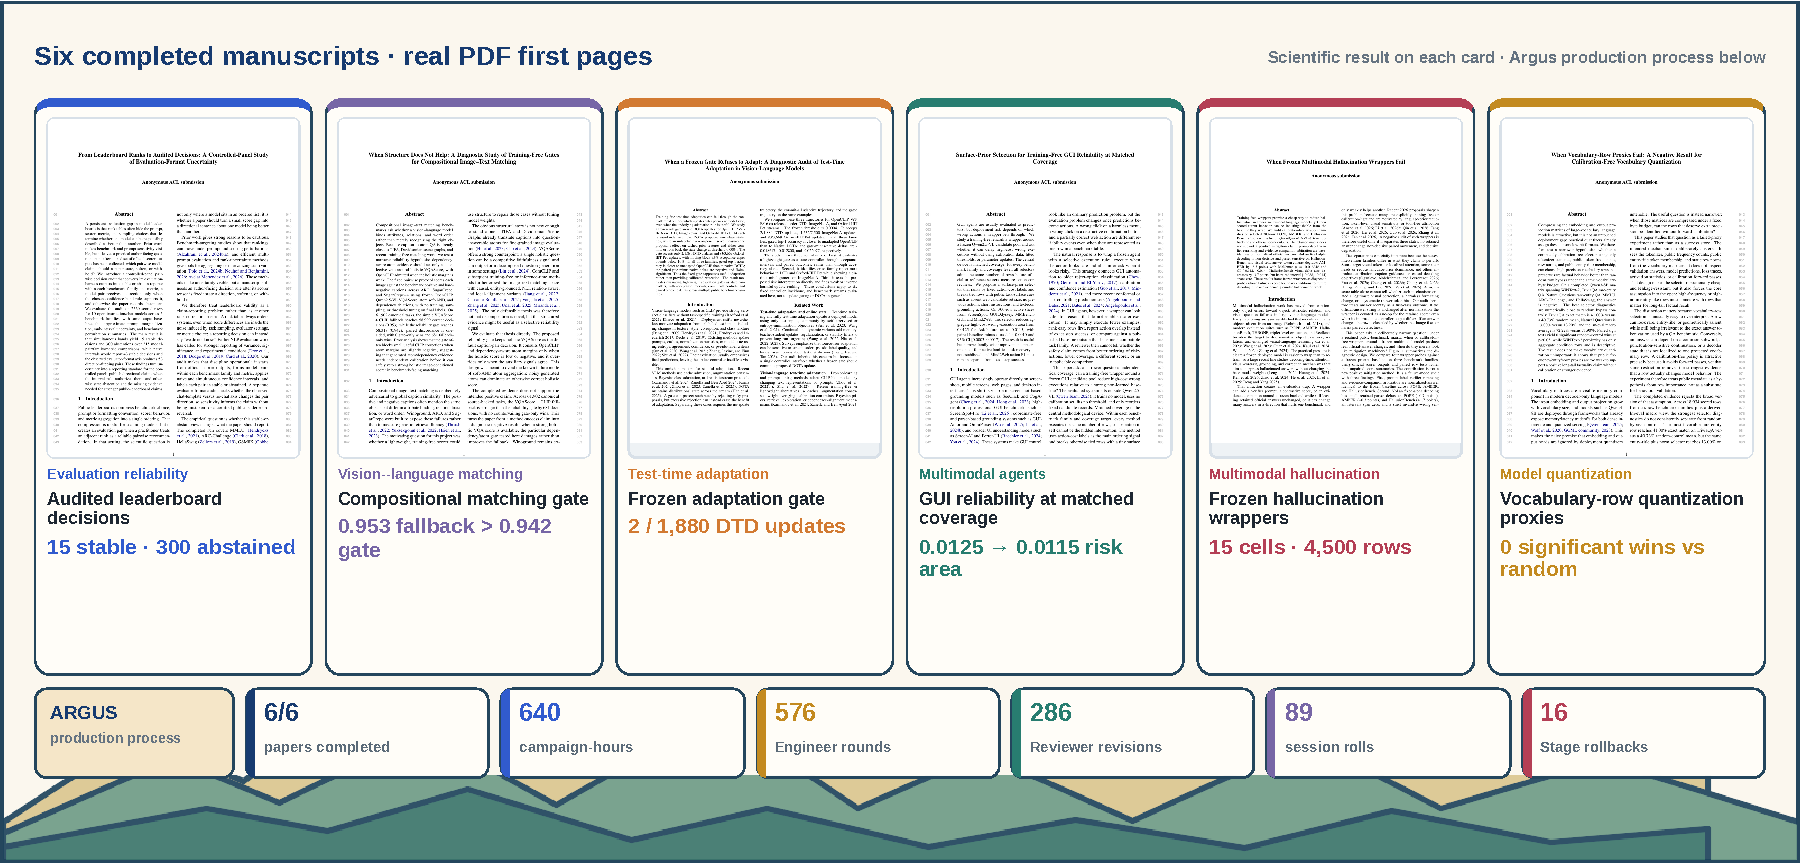
\includegraphics[width=\linewidth]{figures/paper_case_study.pdf}
  \caption{One recurrent runtime, six scientific outputs. Panel (a)
  schematizes the four role authorities around persistent research state. Panel
  (b) reports the research topic and principal measured finding from each
  final manuscript. The bottom strip aggregates structured runtime events across
  the six campaigns. The mechanism panel is schematic; the paper findings and
  process counts are measured. AAAI and ACL labels denote formatting rather than
  venue acceptance.}
  \label{fig:paper-case-study}
\end{figure}

The trajectories are inconsistent with a one-pass account of autonomous paper
writing. Each manuscript states a scoped research question and a task-native
outcome rather than merely presenting a generated document. The portfolio includes
uncertainty-aware leaderboard reporting, a failed compositional gate, an
over-restrictive adaptation controller, a narrow GUI reliability gain, a
failure-mode audit of multimodal wrappers, and a negative result for static
quantization proxies. Several projects therefore become diagnostic or negative
results after their original positive hypothesis fails. Reviewer-gated state makes
that scientific pivot explicit instead of silently replacing the failed branch.

Figure~\ref{fig:paper-case-trajectory} resolves the multimodal-hallucination
campaign in greater detail. During a dense 12-hour search window, seven rollback
decisions reject baseline coverage or proposed mechanisms that are unreproduced,
base-identical, or missing their preregistered signal. Planner then changes the
claim from a positive mitigation method to a diagnostic negative-results audit.
Engineer completes a five-method by three-benchmark matrix with 4,500
official-scored rows; Reviewer binds the resulting no-op and degradation claims to
those outputs. Two later submission checks return the project to benchmark to
repair scorer provenance and GPU telemetry before the final 10-page AAAI-formatted
package completes the pipeline.

\begin{figure}[H]
  \centering
  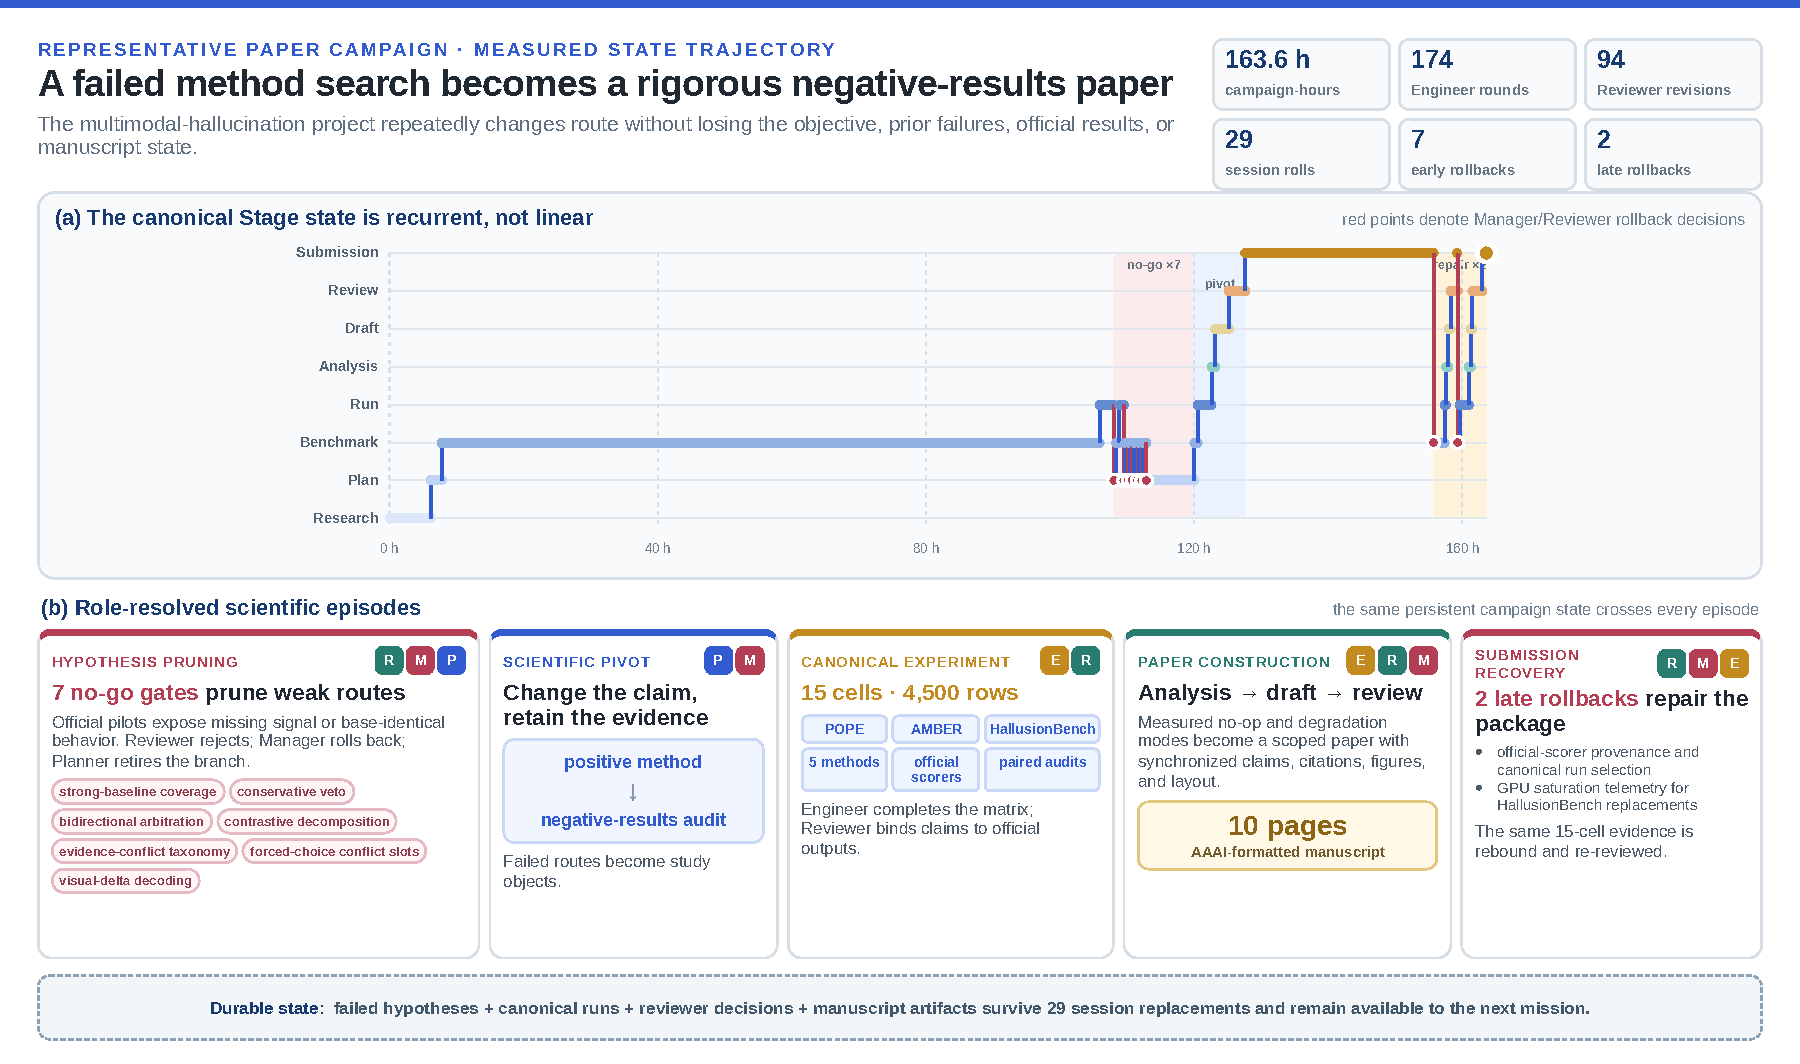
\includegraphics[width=\linewidth]{figures/paper_case_trajectory.pdf}
  \caption{Representative 163.6-hour paper-production trajectory. The upper panel
  plots the actual Manager-controlled Stage state against elapsed campaign-hours;
  red points mark rollback decisions. Seven early no-go rollbacks prune weak method
  routes before a negative-results scope pivot, and two submission-to-benchmark
  rollbacks repair the final evidence package. The lower panel identifies the role
  actions and retained artifacts at each scientific episode. The canonical
  experiment contains 15 method--benchmark cells and 4,500 official-scored rows;
  29 session rolls do not reset the campaign state.}
  \label{fig:paper-case-trajectory}
\end{figure}

The process layer is similarly nontrivial. Even the shortest case requires 28
Engineer rounds, 19 Reviewer revisions, and 13 session rolls over 20.8 hours. The
two AAAI-formatted cases finish as 10-page anonymous submissions, while the four
ACL-formatted cases contain 10--13 pages. Across all six projects, the retained
academic, layout, and infrastructure histories contain
\PaperCaseReviewSnapshots{} automated review snapshots. These are process records
rather than external assessments of paper quality.

The case study also exposes a consistency failure. The compositional-matching
pipeline reaches a complete submission Stage and produces its final PDF, while the
last stored assurance object remains \code{BLOCKED} on a Manager-stage authority
check. This discrepancy does not change the paper artifact, but it shows that
derived certification state can lag the canonical pipeline state. Public release
automation should reconcile those two views before presenting assurance as a final
verdict.

\section{Analysis and Discussion}
\label{sec:discussion}

\subsection{System-Level Performance}

The seven-benchmark suite shows one runtime operating across software repair,
GPU-kernel optimization, model training, research tasks, data synthesis, and
mathematical proof. On SWE-Bench Pro, \systemname reaches approximately 78\%
accuracy compared with 59\% for Direct Copilot at 1.41$\times$ aggregate Tokens.
The comparison pairs additional computation for planning, execution, and review
with a 19-point accuracy difference.

The longitudinal run shows how this cost changes with accumulated state. Mature
W19--22 uses 21\% fewer solve input Tokens and 15\% less active time per task than
startup W1--6. The curve remains non-monotone: W13--18 combines low Token use with
longer execution, while W23--24 contains a late concentration of difficult tasks. The operating profile changes
over time as shared state expands, while task-dependent variation remains visible.

\subsection{Reviewer as Selective Error Correction}

The Reviewer requests revision on 43 SWE-Bench Pro tasks. After another Engineer
round, 34 pass the official verifier and 22 complete the stricter
\code{continue}$\rightarrow$revision$\rightarrow$\code{done} loop. These trajectories
show the Reviewer functioning as an error-correction stage rather than a terminal
commentary layer.

Reviewer routing is adaptive: Reviewer-routed tasks use more Tokens and active time
than self-reviewed tasks. The observed routing concentrates independent review on
the more resource-intensive part of the workload.

\subsection{Autonomous Research Production}

The six-paper case study extends the endpoint results into a complete research
lifecycle. All six canonical pipelines reach submission completion across six
domains and two venue formats, but none follows a one-pass path. Reviewer revision
verdicts, Stage rollbacks, and session rolls are common rather than exceptional.
The final manuscripts therefore demonstrate persistence across research framing,
experimentation, writing, review, and packaging---not merely the ability to emit
paper-like prose.

The multimodal-hallucination trace makes the control mechanism explicit. Reviewer
gates prevent seven weak method routes from being scaled into an unsupported
positive claim; Planner reframes the accumulated failures as a diagnostic study;
Engineer then completes the 15-cell canonical matrix; and Manager accepts two late
rollbacks when submission checks expose scorer-provenance and telemetry defects.
The role separation therefore changes the scientific trajectory: failure is
retained as information, while only reviewed state controls the next Stage.

The case also separates artifact completion from process certification. Five final
assurance snapshots pass; the compositional-matching project retains a stale blocked
assurance snapshot after its canonical pipeline and final PDF complete. This is a
useful systems distinction: derived quality metadata must be reconciled with the
authoritative Stage state before it can serve as a public certificate.

\subsection{Persistent State and Process Data}

The long-lived object in \systemname is the campaign state rather than a provider
transcript. Accepted results, failed routes, tools, skills, and current blockers
remain available after session and process restarts. Equation~\ref{eq:process-data}
formalizes the information advantage of this record, while
Equation~\ref{eq:process-compression} explains why the runtime keeps both a complete
event history and a bounded working checkpoint.

This mechanism gives concrete meaning to \emph{compounding intelligence}. The base
model remains fixed, but each accepted mission changes the starting point of later
work. The SWE-Bench Pro trajectory measures the resource profile across this
accumulation, and the mathematical campaign shows later theorem missions consuming
earlier definitions, bounds, rejected routes, and bridge lemmas.

\subsection{From Runtime Learning to Model Training}

The same trajectories can be transformed into supervised examples, preference
pairs, and reinforcement-learning transitions. AgentInstruct, Agent-FLAN, and
Agent Lightning provide complementary mechanisms for this conversion
~\citep{mitra2024agentinstruct,chen2024agentflan,luo2025agentlightning}.
\systemname contributes a structured source stream linking objectives, tool actions,
measurements, revisions, and retained-state updates. A future training stage can use
this stream to internalize recurring planning and verification patterns while the
runtime continues to provide long-horizon coordination.

\subsection{Vertical Research in Mathematics}

The Erd\H{o}s--Gy\'arf\'as campaign exposes the four-role organization at research
depth. The Manager preserves the objective and stage, the Planner converts the
current frontier into bounded theorem tasks, the Engineer produces proofs and
computational checks, and the Reviewer controls admission into durable state.

The campaign retains one falsified route and six accepted theorem-frontier updates.
Later missions improve a bound and close two graph-realizability gaps by starting
from the reviewed ledger rather than restarting from the original conjecture. This
is the same runtime mechanism seen in software repair, applied to a domain where
progress is expressed through definitions, lemmas, counterexamples, and proofs.

\subsection{Connecting Theory and Results}

Table~\ref{tab:theory-results} connects the process-to-capability model to the
measurements reported in Sections~\ref{sec:results} and~\ref{sec:vertical-trace}.

\begin{table}[H]
\centering
\scriptsize
\renewcommand{\arraystretch}{1.12}
\begin{tabularx}{\linewidth}{@{}p{2.4cm}p{3.55cm}p{2.55cm}X@{}}
\toprule
\rowcolor{papersand}
\textbf{Theory component} & \textbf{Measurement} & \textbf{Observed result} & \textbf{Interpretation} \\
\midrule
Process-data dominance & Mathematical trajectory & One dead route and six dependent theorem updates & The retained process changes the starting state of later missions. \\
Review gate & 43 Reviewer revision requests & 34 verifier recoveries; 22 strict rescues & Independent review redirects initially unacceptable work into another implementation round. \\
Reuse value $G_K$ & Startup W1--6 versus mature W19--22 & 21\% fewer solve input Tokens; 15\% less active time & Later operation reaches a lower resource regime while shared state expands. \\
Recovery under persistent state & Paper-production trajectory & Seven early no-go rollbacks, two late submission repairs, and 29 session rolls & The campaign changes hypothesis and repairs evidence without losing accepted results or restarting the manuscript. \\
Token conversion & Rounds 12--17 role attribution & 56.0\% reasoning, 55.4\% verification, and 55.6\% action direct shares & The research trace separates frontier work, coordination, and interrupted work. \\
\bottomrule
\end{tabularx}
\caption{Connection between the process-to-capability theory and measured system
behavior. Detailed substitutions appear in Appendix~\ref{app:formula-instantiation}.}
\label{tab:theory-results}
\end{table}

\section{Limitations and Future Work}
\label{sec:limitations}

\paragraph{The benefit of user-guided pivots is not yet causally evaluated.}
The retained traces show evidence-backed changes to operational objectives,
constraints, and verification obligations, but they do not include a prospective
human-subject comparison. We therefore do not claim that the current experiments
prove improved expert understanding. A direct evaluation should compare
\systemname with fixed-prompt agents and ordinary interactive assistants on expert
calibration, time to identify the binding constraint, quality of contract revisions,
number of repeated misconceptions, and final task value.
Likewise, internal-expert observations about appropriate stopping motivate the
analysis in Section~\ref{sec:discussion} but are not reported as a satisfaction rate
or comparative user-study result.

\paragraph{Contract refinement can still fail.}
Evidence, provenance, and authority reduce goal drift but do not eliminate it. An
expert may approve a poorly framed tradeoff, Reviewer may miss a contradiction, or
the recorded standing intent may omit a tacit requirement. Future work should test
adversarial contract changes, invariant-preservation checks, disagreement handling,
and rollback of harmful refinements. High-impact domains also require explicit
human sign-off policies rather than relying on Manager judgment alone.

The task-contract notation is an analytical abstraction over several persisted
runtime surfaces, not a claim that the implementation currently exposes one atomic
$K_t$ object or a universal automated user-admission API. A future implementation
should unify those fields and make authorization and rollback directly queryable.

\paragraph{Verification is only as sound as its evidence boundary.}
An executable test, formal checker, benchmark, or model Reviewer can all encode the
wrong property. The framework makes verifier revision possible but does not confer
correctness automatically. System-verification studies should separately seed bugs
in code, bugs in specifications, and mismatches between them, then measure whether
the runtime localizes the faulty side instead of merely making the current checker
pass.

\paragraph{Attribution and task sequence.}
The SWE-Bench Pro experiment compares the complete \systemname runtime with Direct
Copilot. Reviewer routing is adaptive, the 22 Waves follow one task order, and
per-Wave Direct-Copilot Token/time records are unavailable. The current results
therefore characterize whole-system behavior over this sequence. Matched
frozen-state runs, randomized task orders, and randomized review routing will
separate the contributions of persistent state, role separation, and review.

\paragraph{Generality across models, domains, and evaluators.}
The seven benchmark arenas use different metrics, hardware, and execution
protocols, while the mathematical analysis follows one vertical campaign. Results
are interpreted in their native units rather than combined into a universal score.
Repeated campaigns, additional backbones, and external domain review will measure
how the runtime transfers across task families and research standards.

\paragraph{Metric calibration and model transfer.}
The efficiency analysis labels whole role calls by mission purpose; finer segment
labels would sharpen the reasoning, action, and verification factors. Reviewer
sensitivity and false-acceptance rate require randomized routing with an external
verifier, and the counterfactual reuse value $G_L$ requires paired future tasks with
and without a state update. The runtime-to-model path is currently a training
direction: held-out trajectory splits and scaffold-removal studies will measure how
much of the long-horizon control loop can be internalized by the model.

\paragraph{Paper-production trajectories are observational.}
The six paper projects were selected from one shared research environment and do
not include a matched human-authoring baseline. Campaign-hours overlap in calendar
time, stored review snapshots are model-generated rather than independent human
reviews, and runtime logging evolved across projects. The case study therefore
supports end-to-end lifecycle and recovery claims, not paper acceptance, scientific
novelty, or superiority to human research teams. Recorded costs in the public data
also exclude utility calls without a priced event.

\paragraph{Artifact evidence levels.}
The FLA case is linked to a public merged pull request and archived timing and
correctness evidence. The ACE-1 description and 75/80 score come from the supplied
project presentation; the report bundle does not include enough raw PPA and
throughput material for independent recomputation. ACE-1 is therefore evidence of
an artifact-producing chip-design workflow, not a reproduced SOTA comparison.

\section{Conclusion}
\label{sec:conclusion}

We introduced \system{}, a persistent runtime for long-horizon autonomous research.
The system decomposes a campaign into bounded missions, separates planning,
execution, and acceptance across explicit roles, records an append-only experiment
trace, and retains reviewed experience as inspectable runtime state around a fixed
model. This organization moves continuity from an unbounded model transcript into
recoverable project state.

The current public record spans six benchmark arenas and 41 de-duplicated research
artifacts across six programs. These results demonstrate operational breadth and
competitive task-level outcomes. The next step is not a broader headline claim, but
stronger causal and reproducibility evaluation: controlled ablations, broader task
coverage, calibrated review, and longitudinal measurements of what the
runtime actually retains.


\clearpage
\appendix
\section{Implementation Interfaces and Lifecycle}
\label{app:interfaces}

This appendix records source-level contracts and operational defaults that are
useful for reproduction but too detailed for the main argument. The lifecycle is
specified directly through role contracts, outcome states, persistence surfaces,
and guard conditions; no additional conceptual diagram is required.

\subsection{Role Contracts}

The Manager front door uses one grounded model decision to emit six structured
axes: \code{CONFIG}, \code{CONTROL}, \code{ROUTE}, \code{LIFETIME},
\code{FAST\_REPLY}, and \code{NAME}. A \code{CONTROL: NO\_DISPATCH} result is
authoritative and fails closed: the bridge may provide a read-only response but may
not enqueue work. The Manager is also the sole writer of the current campaign
stage.

The Planner produces \code{TaskSpec} objects with explicit scope, optional DAG
dependencies, and impact score. It authors and applies stage \code{checklist\_ops};
the Reviewer can send \code{checklist\_feedback} but does not edit the checklist.
The Engineer receives reservation-derived provider fences through
\code{RunnerOptions} and returns a \code{RunnerResult} with a call identifier,
usage-presence flags, cost, and pricing status. The Reviewer returns a
\code{ReviewDecision} whose central fields are listed in
Table~\ref{tab:review-interface}.

\begin{table}[H]
\centering
\footnotesize
\begin{tabularx}{\linewidth}{@{}p{3.3cm} X@{}}
\toprule
\textbf{Reviewer field} & \textbf{Meaning} \\
\midrule
\code{status} & \code{done}, \code{continue}, or \code{blocked}; the mission-level completion verdict \\
\code{progress\_class} & \code{decision}, \code{evidence}, \code{setup\_only}, \code{artifact\_sync\_only}, or \code{none} \\
\code{next\_action} & Concrete action for the next Engineer round \\
\code{operator\_question} & At most one human-facing blocking question \\
\code{scope, checklist} & Structured final-submission gate, evaluated fail-closed \\
\code{skill\_ops, wiki\_ops} & Reviewer-authored retained-state edits \\
\code{backend\_unavailable} & Infrastructure failure, never interpreted as a scientific \code{continue} \\
\bottomrule
\end{tabularx}
\caption{Abridged Reviewer interface from \srcpath{core/models.py} and
\srcpath{reviewer/reviewer\_schema.json}.}
\label{tab:review-interface}
\end{table}

\subsection{Outcome Taxonomy}

Every mission produces an explicit outcome:

\begin{itemize}
  \item \textbf{Terminal:} \code{done}, \code{max\_rounds}, \code{blocked},
    \code{no\_progress}, \code{error}, and \code{budget\_exhausted}.
  \item \textbf{Paused:} \code{paused\_budget},
    \code{paused\_provider\_cooldown}, \code{paused\_provider\_fence},
    \code{infra\_blocked}, \code{research\_incomplete},
    \code{paused\_no\_breakthrough}, and
    \code{exhausted\_current\_methods}.
  \item \textbf{Control transfer:} \code{replan\_requested}; the item returns to
    pending and passes through the normal Planner gate rather than being counted as
    completed or failed.
\end{itemize}

\section{Persistence and Context Management}
\label{app:persistence}

The global state root defaults to \code{\textasciitilde/.argus-skill/} and can be
overridden by \code{ARGUS\_SKILL\_HOME}. Each project is stored under a fingerprinted
subdirectory. Table~\ref{tab:persisted-state} lists the principal files.

\begin{table}[H]
\centering
\footnotesize
\begin{tabularx}{\linewidth}{@{}p{3.0cm} p{2.0cm} X p{1.75cm}@{}}
\toprule
\textbf{Path} & \textbf{Owner} & \textbf{Content} & \textbf{Mutation} \\
\midrule
\code{events.jsonl} & record plane & Canonical typed-event timeline & append-only \\
\code{backlog.jsonl} & scheduler & Pending, running, completed, and superseded tasks & atomic claim / CAS \\
\code{continuous.json} & Manager / scheduler & Standing objective, route, lifetime, and identity & atomic rewrite \\
\code{inbox.jsonl} & operator & Operator messages and answers & append + drain \\
\code{checkpoint.json} & Reviewer & Hard-capped cross-session working state & atomic rewrite \\
\code{daemon.pid} & daemon & Per-project concurrency lock & exclusive \\
\code{daemon.status.json} & daemon & Liveness and handoff status & rewrite \\
\code{skills/} & Reviewer / operator & Versioned reusable skills & versioned \\
\bottomrule
\end{tabularx}
\caption{Principal persisted state. The event tape is the canonical timeline;
other files are working state or materialized views.}
\label{tab:persisted-state}
\end{table}

The checkpoint contains the goal, verified work, tried-and-failed approaches, one
open blocker, the next step, and bounded environment facts. The Engineer proposes a
handoff, and the Reviewer validates and writes the canonical \code{checkpoint.json}.
Python-level item and character caps prevent it from becoming an append-only
transcript. A missing or malformed candidate checkpoint preserves the last valid
state rather than clearing memory.

By default, each role thread is rolled after three rounds on that thread or when the
preceding call reports at least 1.5 million input tokens. The next session is
re-seeded from the checkpoint. These limits are configurable and disable at zero.
The design keeps provider prefix caching useful over short windows while preventing
unbounded compaction loops.

Unattended execution is wrapped by
\srcpath{daemon/life\_worker.py} (roughly 1,800 lines). The worker drains on
\code{SIGTERM} or \code{SIGINT} at a mission boundary. Source upgrades use a
blue/green self-handoff with a bounded generation count and persisted identity
consisting of the objective hash, vertical, and lineage generation. A resume adopts
only a matching identity; otherwise the Manager must perform a fresh division.

\section{Run Records and Provenance}
\label{app:evidence-map}

\subsection{Event Catalog and Call Correlation}

The canonical catalog contains \textbf{112 typed event types} across
\textbf{11 categories}; \textbf{75} event types carry validated payload schemas in
\srcpath{core/event\_catalog.py}. Table~\ref{tab:event-taxonomy} gives the category
counts. The event \code{research.achievement.certified} is the sole authoritative
record of a verified achievement.

\begin{table}[H]
\centering
\footnotesize
\begin{tabularx}{0.86\linewidth}{@{}p{2.3cm} r X@{}}
\toprule
\textbf{Category} & \textbf{Count} & \textbf{Representative content} \\
\midrule
Lifecycle & 40 & Loop, round, mission, and budget-reservation events \\
Skill & 20 & Match, distillation, use, and outcome events \\
Wiki & 17 & Source ingest, page synthesis, promotion, and validation \\
Planner & 9 & Planning start, tasks, waiting contracts, and verdicts \\
Research & 7 & Achievement certification and research status \\
Agent I/O & 5 & Provider-call start, stream, and completion \\
Daemon & 5 & Start, stop, handoff, and status \\
Idea & 3 & Idea lifecycle \\
Provider & 3 & Provider request start, completion, and denial \\
Usage & 2 & Presence-aware usage and cost \\
Operator & 1 & Operator inbox event \\
\bottomrule
\end{tabularx}
\caption{Event taxonomy in the current implementation.}
\label{tab:event-taxonomy}
\end{table}

Every provider call receives a \code{call\_id} at
\srcpath{core/run\_gateway.py}. The identifier is written to the event tape and
returned in the runner result, allowing Reviewer prompts and later audits to locate
the exact execution record. Usage-presence booleans distinguish a genuine zero from
provider-omitted accounting.

\subsection{Credential Handling and Optional Signing}

\srcpath{core/secret\_guard.py} redacts authorization headers, API-key patterns,
provider tokens, and generic key/value secrets before event or artifact copies are
persisted for downstream use. A redaction emits \code{round.secret\_redacted}; a
scan error or uncovered oversized artifact blocks unconditional certification.

An optional Ed25519 signing path in \srcpath{team/result\_provenance.py} supports
isolated-scorer teammate results. It is off by default and is not used for the
results reported here.

\subsection{Artifact-Digest Records}

The nanoGPT speedrun row points to logical project
\nolinkurl{nanogpt-speedrun-h100} and artifact
\nolinkurl{candidate_mlp_post_only_hybrid_n10_20260617T152904Z}. Its verifier
records \code{valid=true}, $N{=}10$, validation loss $3.2776$, one-sided
$p(\mathrm{mean}<3.28)=0.004007$, training time $79.77\pm0.06$ seconds, and
\code{seal=ok}. The nanochat B200 row points to logical project
\nolinkurl{nanochat-mission-b200} and artifact
\nolinkurl{a374_tailweighted_boundary_mixed_readout_data_bundle}; its frozen scorer
exits 0 with \code{MEAN\_VAL\_BPB=0.963634} and a valid SM100 flash-attention kernel.
The result JSON stores source/result hashes and verifier excerpts, but not the
external bytes.

Both public pages were retrieved at \code{2026-07-14T12:29:51Z}. Their complete
raw-HTML SHA-256 values are recorded in \srcpath{evidence/website\_results.json}
and \srcpath{evidence/paper\_inventory.json} rather than typeset inline.

\subsection{Source Map}

\begin{table}[H]
\centering
\footnotesize
\begin{tabularx}{\linewidth}{@{}p{4.1cm} X@{}}
\toprule
\textbf{Subsystem} & \textbf{Primary source path(s)} \\
\midrule
Runtime composition and roles & \code{manager/}, \code{planner/}, \code{engineer/}, \code{reviewer/}, \code{loop.py} \\
Mission lifecycle and daemon & \code{life/supervisor/\_core.py}, \code{daemon/life\_worker.py}, \code{daemon/handoff.py} \\
State and memory & \code{core/paths.py}, \code{apps/\_runtime.py}, \code{engineer/checkpoint.py}, \code{life/memory.py} \\
Execution and budgets & \code{core/run\_gateway.py}, \code{core/pricing.py}, \code{core/usage.py}, \code{core/provider\_quota.py} \\
Reliability guards & \code{engineer/runner.py}, \code{regime\_jump/} \\
Records and integrity & \code{core/event\_catalog.py}, \code{core/secret\_guard.py}, \code{skills/provenance.py} \\
Cockpit and API & \code{webapi/server.py}, \code{frontend/tui/}, \code{frontend/web/} \\
Public results & \code{technical\_report/evidence/website\_results.json}, \code{paper\_inventory.json} \\
\bottomrule
\end{tabularx}
\caption{Repository map for implementation and reported results.}
\label{tab:source-map}
\end{table}

\section{Reliability, Budgets, and Deployment}
\label{app:reliability}

The guards in Table~\ref{tab:guards} define the long-running execution envelope.
They are task-agnostic: they constrain activity and resource use, while the Reviewer
remains responsible for scientific judgment.

\begin{table}[H]
\centering
\footnotesize
\begin{tabularx}{\linewidth}{@{}p{2.75cm} X p{1.3cm} p{1.55cm}@{}}
\toprule
\textbf{Guard} & \textbf{Trigger and action} & \textbf{Default} & \textbf{Live-call interrupt} \\
\midrule
Backend failure & Consecutive failures $\rightarrow$ backoff, then error & 2 / 15 s & no \\
No-progress bail & Consecutive rounds with no Engineer message & 2 & no \\
Decision stall & Consecutive nondecision review classes $\rightarrow$ end & 4 & no \\
Decision-progress budget & Time since last decision/evidence $\rightarrow$ end & 1,800 s & no \\
Soft round escalation & Ask Reviewer to return \code{blocked} & 12 & no \\
Hard round escalation & Force terminal \code{blocked} & 24 & no \\
Effective-progress watchdog & No file change or non-token event & 3,600 s & yes \\
Runner hard-idle & No runner activity & 3,600 s & yes \\
In-round compaction limit & Repeated automatic compactions & 3 & yes \\
\bottomrule
\end{tabularx}
\caption{Default reliability guards in \srcpath{engineer/runner.py}. Thresholds are
environment-overridable and disable at zero where applicable.}
\label{tab:guards}
\end{table}

The canonical \code{resolve\_budget\_caps} path in \srcpath{core/knobs.py} resolves
a per-mission preflight cap of \$30, a per-project daily cap of \$180, a global
daily cap of \$30, and at most two active daemons across projects. A positive global
cap is enforced; setting it to zero disables it. Calls reserve budget before
execution and settle or release the reservation afterward. Unpriced calls and
provider-fence breaches produce explicit blocked events rather than fabricated
costs.

Supervised background jobs maintain their own health cadence and report terminal
outcomes through the operator inbox. An Engineer may explicitly emit
\code{WAIT\_FOR\_SUBAGENT} for a healthy self-watched job; otherwise the request
falls back to a normal reviewed round. The GPU lease tool is explicit rather than
automatic: \code{gpu\_lease run -- <cmd>} releases parked devices, records a lease
for the command lifetime, and restores the keep-alive only when no competing lease
remains.

The intended deployment is a per-project \code{systemd --user} service. It runs the
daemon in the foreground, uses \code{SIGTERM}, allows up to 1,800 seconds for a clean
mission-boundary drain, and restarts under a bounded service policy. Sandboxed
builder roles are confined to the project working directory and may not write the
global state root or provider configuration. The terminal and web cockpits read the
same event tape; mutating commands and sensitive global views require an
authorization token when configured.

\section{Notation and Figure Provenance}
\label{app:notation}

\begin{table}[H]
\centering
\footnotesize
\begin{tabularx}{0.88\linewidth}{@{}p{2.5cm} X@{}}
\toprule
\textbf{Symbol} & \textbf{Meaning} \\
\midrule
$o,y_0,f,B$ & Campaign objective, initial artifact, evaluator, and resource budget \\
$\tau_t$ & Mission trajectory $(s_t,a_t,y_t,e_t,r_t)$ \\
$\rho_I(T)$ & Dense-intelligence density over wall-clock horizon $T$ \\
$\dot N_{\mathrm{tok}}$ & Rate of token-mediated reasoning and action \\
$\eta_r,\eta_a,\eta_v$ & Reasoning, action, and verification conversion factors \\
$H_t$ & Runtime state $\{M_t,S_t,A_t,V_t,R_t,Q_t\}$ \\
$E_t$ & Results admitted from mission $t$ \\
$\theta_t$ & Underlying model parameters, fixed in this report \\
$C_t$ & Effective retained capability set \\
$W_t,D_t(d)$ & Capability breadth and depth in domain $d$ \\
$\epsilon$ & Acceptance threshold in the idealized capability-admission rule \\
$V_R(T)$ & Conceptual accumulated research value over horizon $T$ \\
$\Delta I,p_{\mathrm{valid}},\eta_{\mathrm{reuse}}$ & Information gain, validity probability, and reuse efficiency \\
$D_{\mathrm{process}}$ & Retained states, actions, measurements, feedback, and runtime-state deltas \\
\bottomrule
\end{tabularx}
\caption{Notation used in the main text.}
\end{table}

The paper uses three figures, each with a distinct evidentiary purpose. The first-page
teaser, \code{argus\_teaser}, combines the exact objective--runtime--review--state
flow with protocol-scoped public result cards. It is an HTML/CSS vector composition
generated from the committed result JSON by
\srcpath{figures/build\_argus\_teaser.py}; its figure brief, source hashes, editable
HTML, and renderer are recorded in \srcpath{figures/argus\_teaser.json}. The two
empirical figures, \code{public\_results} and \code{paper\_portfolio}, are generated
by \srcpath{figures/build\_report\_figures.py} and digested in
\srcpath{figures/REPORT\_FIGURES.json}. The remaining structural assets in the
repository are intentionally not included: their content is represented more
precisely by equations, tables, and interface definitions in this version.


\clearpage
\bibliographystyle{plainnat}
\bibliography{references}

\end{document}
